\chapter{Elephant Herding Optimization}

\section{Elefanten} 
\begin{figure}[ht]
    \begin{center}
        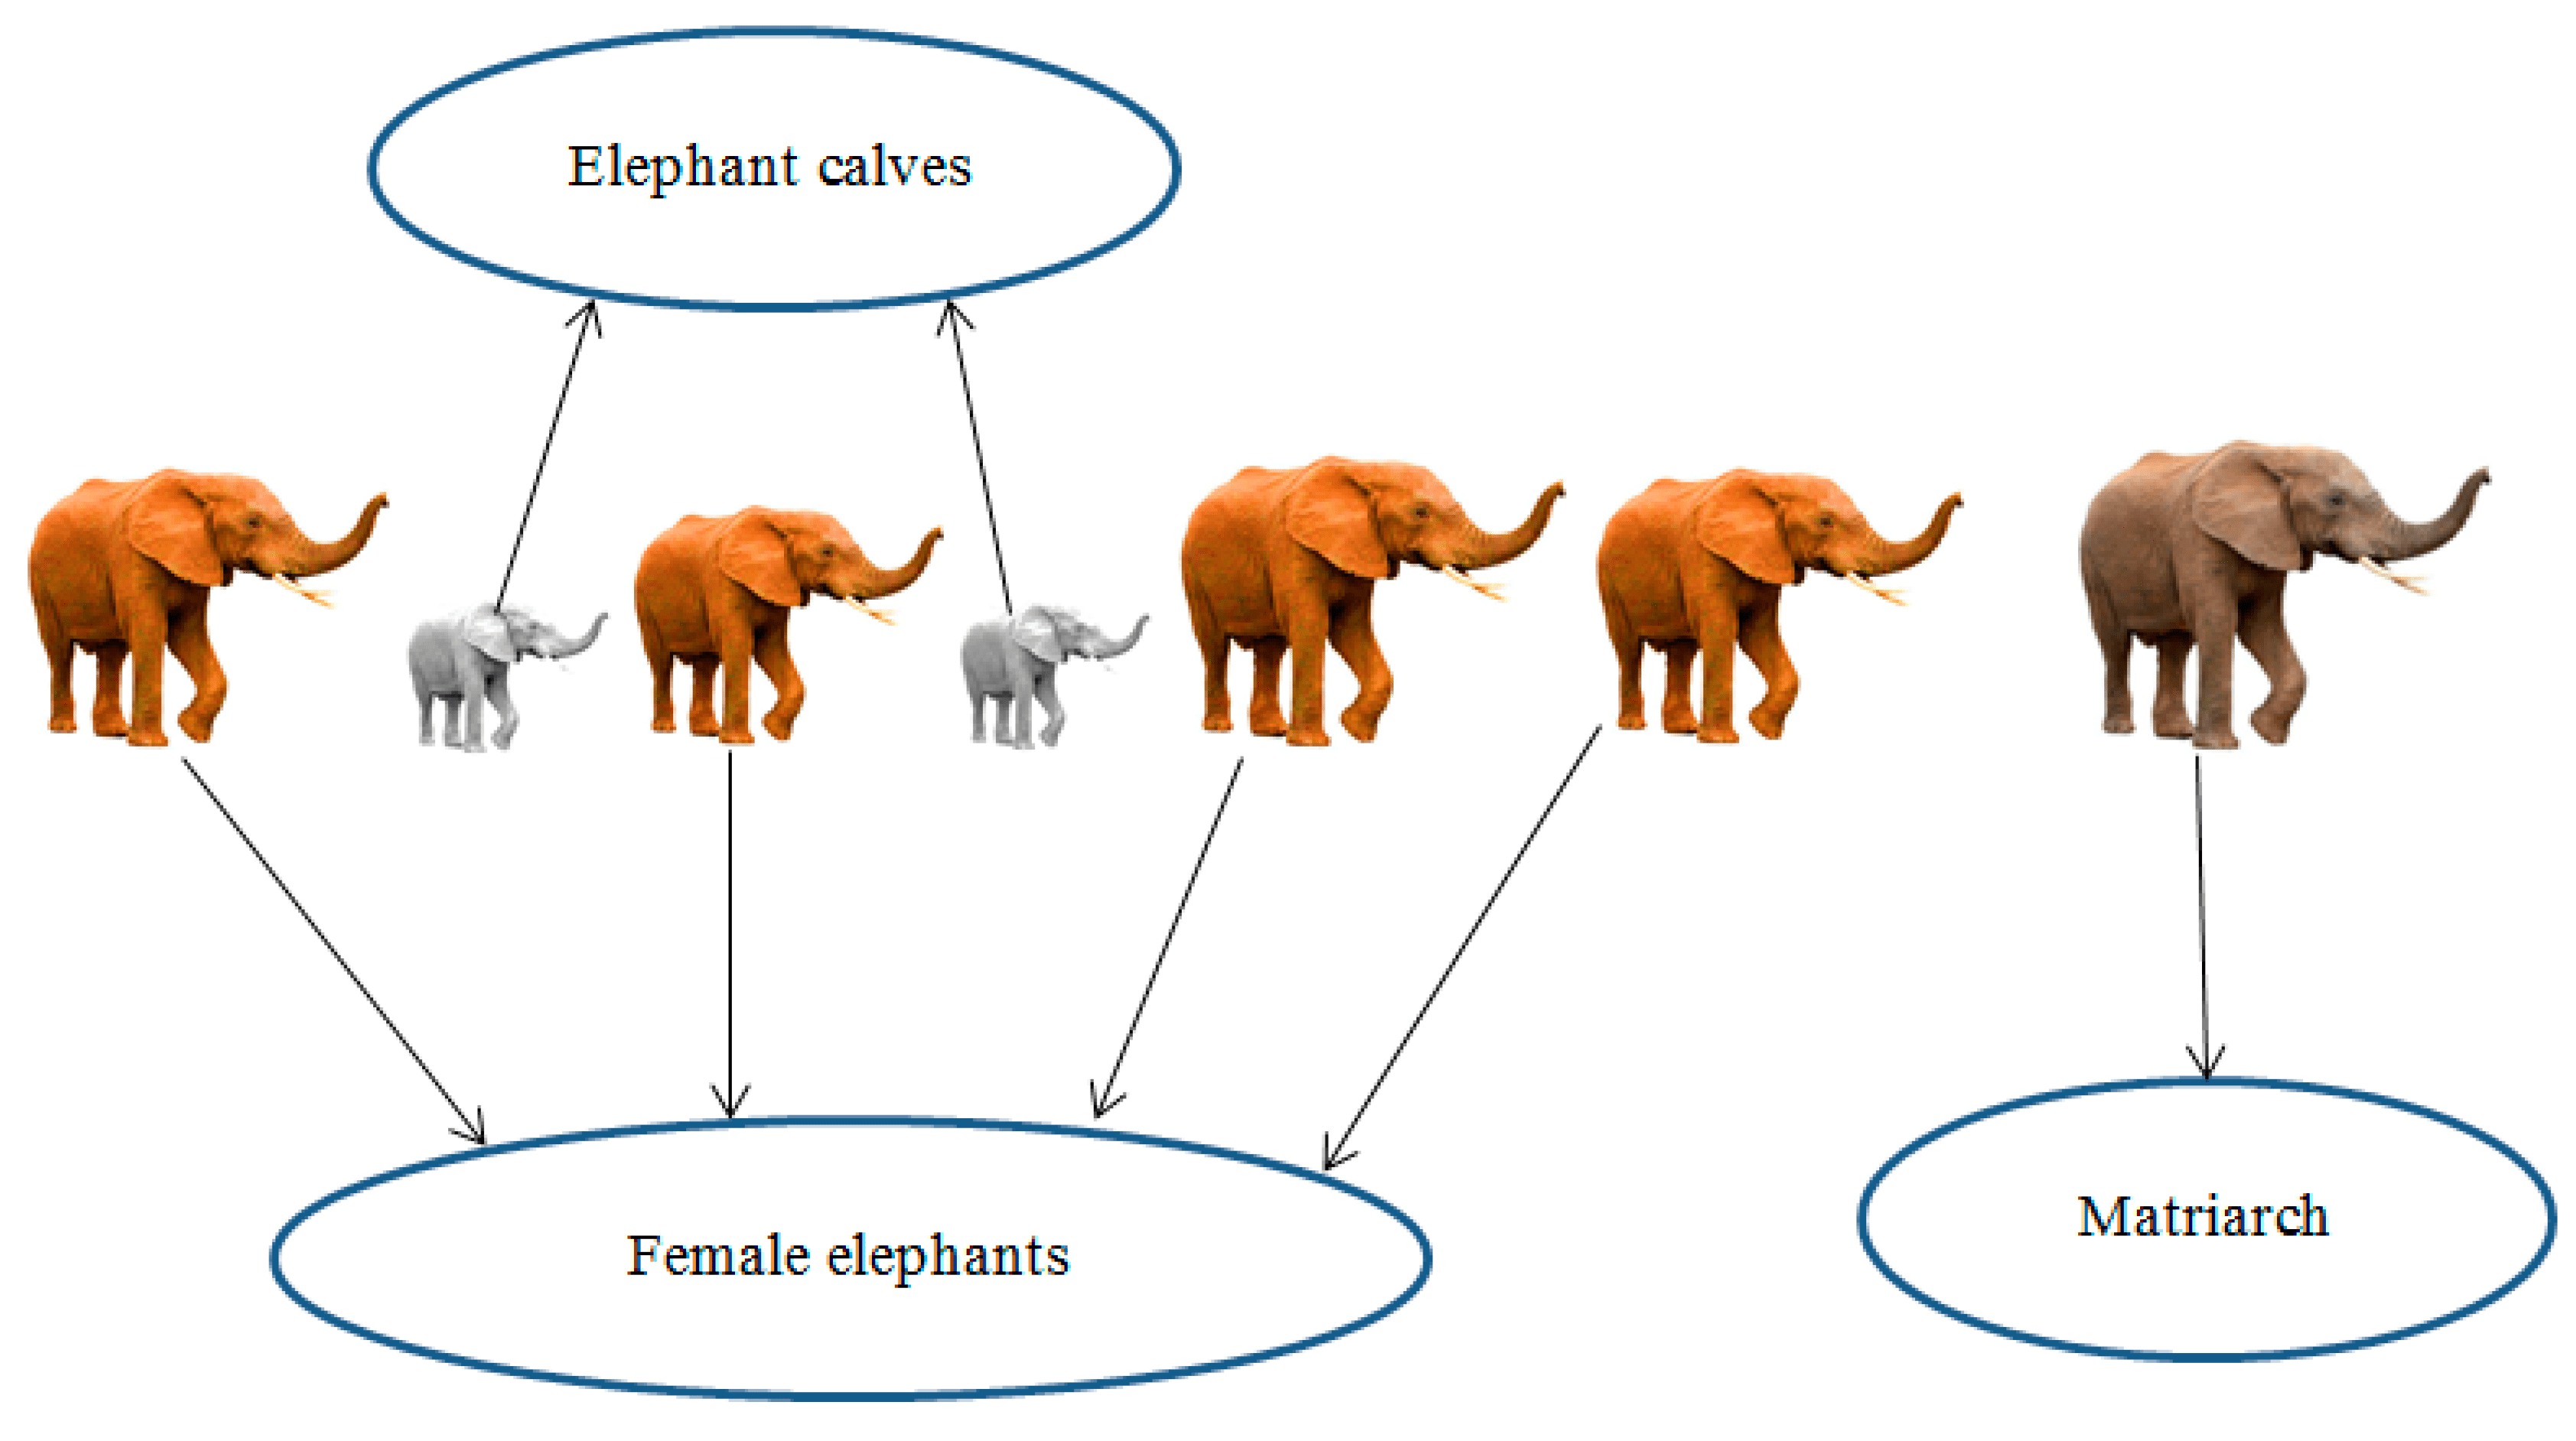
\includegraphics[width=0.7\textwidth]{assets/img/eho_socialstruct.png}
        \caption[EHO Social Structure in a clan]{\cite[Li et al, S.3]{li_lei_alavi_wang_2020}}
        \label{eho_socialstruct}
    \end{center}
\end{figure}
Elefanten sind soziale Tiere mit komplexen Sozialstrukturen. Eine Elefantenherde unterteilt sich in mehrere Clans, die aus weiblichen Tieren und ihren Jungtieren bestehen. Jeder Clan wird von einem Matriarch angeführt, der oft durch die älteste zugehörige Elefantenkuh repräsentiert wird, (siehe \autoref{eho_socialstruct}). Männliche Elefanten leben in Isolation und scheiden mit im Laufe ihres Heranwachsens aus dem Clan aus, \cite[vgl. Wang et al. 2015, S.1]{wang_deb_coelho_2015}. \\
Für den Algorithmus wird die Fortbewegung der Elefanten in Abhängigkeit von ihrem Clan und dem zugehörigen Matriarchen abgebildet und das Ausscheiden der männlichen Tiere aus einem Clan, \cite[vgl. Wang et al, S.1]{wang_deb_coelho_2015}. 

\section{Optimierung}

\subsection{Initialisierung}
Zu Beginn muss die Herde aller Elefanten in Clans aufgeteilt werden, wobei davon ausgegangen wird, dass jeder Clan eine feste Nummer an Tieren beinhaltet, genau einen Matriarchen hat und, dass mit jeder Generation eine feste Anzahl an männlichen Elefanten ihren Clan verlässt, \cite[vgl. Wang et al, S.2]{wang_deb_coelho_2015}. 

\subsection{Clan-Update-Operator} \label{eho_clanUpdate}
Jeder Clan hat einen Matriarchen, dem die Tiere folgen. Daher ist die neue Position $x_{new, ci, j}$ eines Elefanten $j$ in Abhängigkeit von seinem Clan $ci$ und der Position des zugehörigen Matriarchen $x_{best, ci}$ bestimmt (siehe \autoref{calcXNew}). 
\begin{equation}
    x_{new, ci, j} + \alpha \cdot (x_{best, ci} - x_{ci, j}) \cdot r
    \label{calcXNew}
\end{equation}
$x_{ci, j}$ stellt dabei die alte Position des Elefanten und $\alpha \in [0,1]$ einen Skalierungsfaktor, der den Einfluss des Matriarchen ausdrückt. Für $r$ gilt $r \in [0,1]$.\\
\\
Die Position des Matriarchen kann mit \autoref{calcXNew} nicht berechnet werden und es muss \autoref{calcXNewMatriarch} genutzt werden.
\begin{equation}
    x_{new, ci, j} = \beta \cdot x_{center, ci}
    \label{calcXNewMatriarch}
\end{equation}
Die Position des Matriarchen wird mittels der Position des zentralen Tieres $x_{center, ci}$ innerhalb des Clans $ci$ und $\beta \in [0,1]$ repräsentiert einen Skalierungsfaktor. $x_{center, ci}$ kann mittels \autoref{calcXCenter} berechnet werden.
\begin{equation}
    x_{center, ci, d} = \frac{1}{n_{ci}} \cdot \sum_{j=1}^{n_{ci}} x_{ci,j,d}
    \label{calcXCenter}
\end{equation}
Die Position des Tieres $x_{center, ci}$ ist zusätzlich abhängig von der Dimension $d$ mit $1 \leq d \leq D$ und der Anzahl der Tiere in einem Clan $n_{ci}$, \cite[vgl. Wang et al, S.2]{wang_deb_coelho_2015}.

\subsection{Separierungs-Operator} \label{eho_separate}
Der Separierungsprozess beschreibt das Verlassen der männlichen Elefanten des Clans beim Heranwachsen. Die Zahl der Mitglieder bleibt dabei jedoch gleich, die Elefanten werden lediglich ersetzt. Zur Optimierung der Annäherung an das Ziel wird dabei angenommen, dass der Elefant mit der schlechtesten Position ($x_{worst, ci}$) zum Ziel den Clan verlässt (siehe \autoref{calcXWorst}).
\begin{equation}
    x_{worst, ci} = x_{min} + (x_{max} - x_{min} + 1) \cdot rand
    \label{calcXWorst}
\end{equation}
$x_{max}$ und $x_{min}$ stellen die oberen bzw. unteren Grenzen der jeweiligen Dimension dar und $rand \in [0,1]$ eine Zufallszahl, \cite[vgl. Wang et al, S.2]{wang_deb_coelho_2015}.

\subsection{Algorithmus}
\begin{figure}[ht]
    \begin{center}
        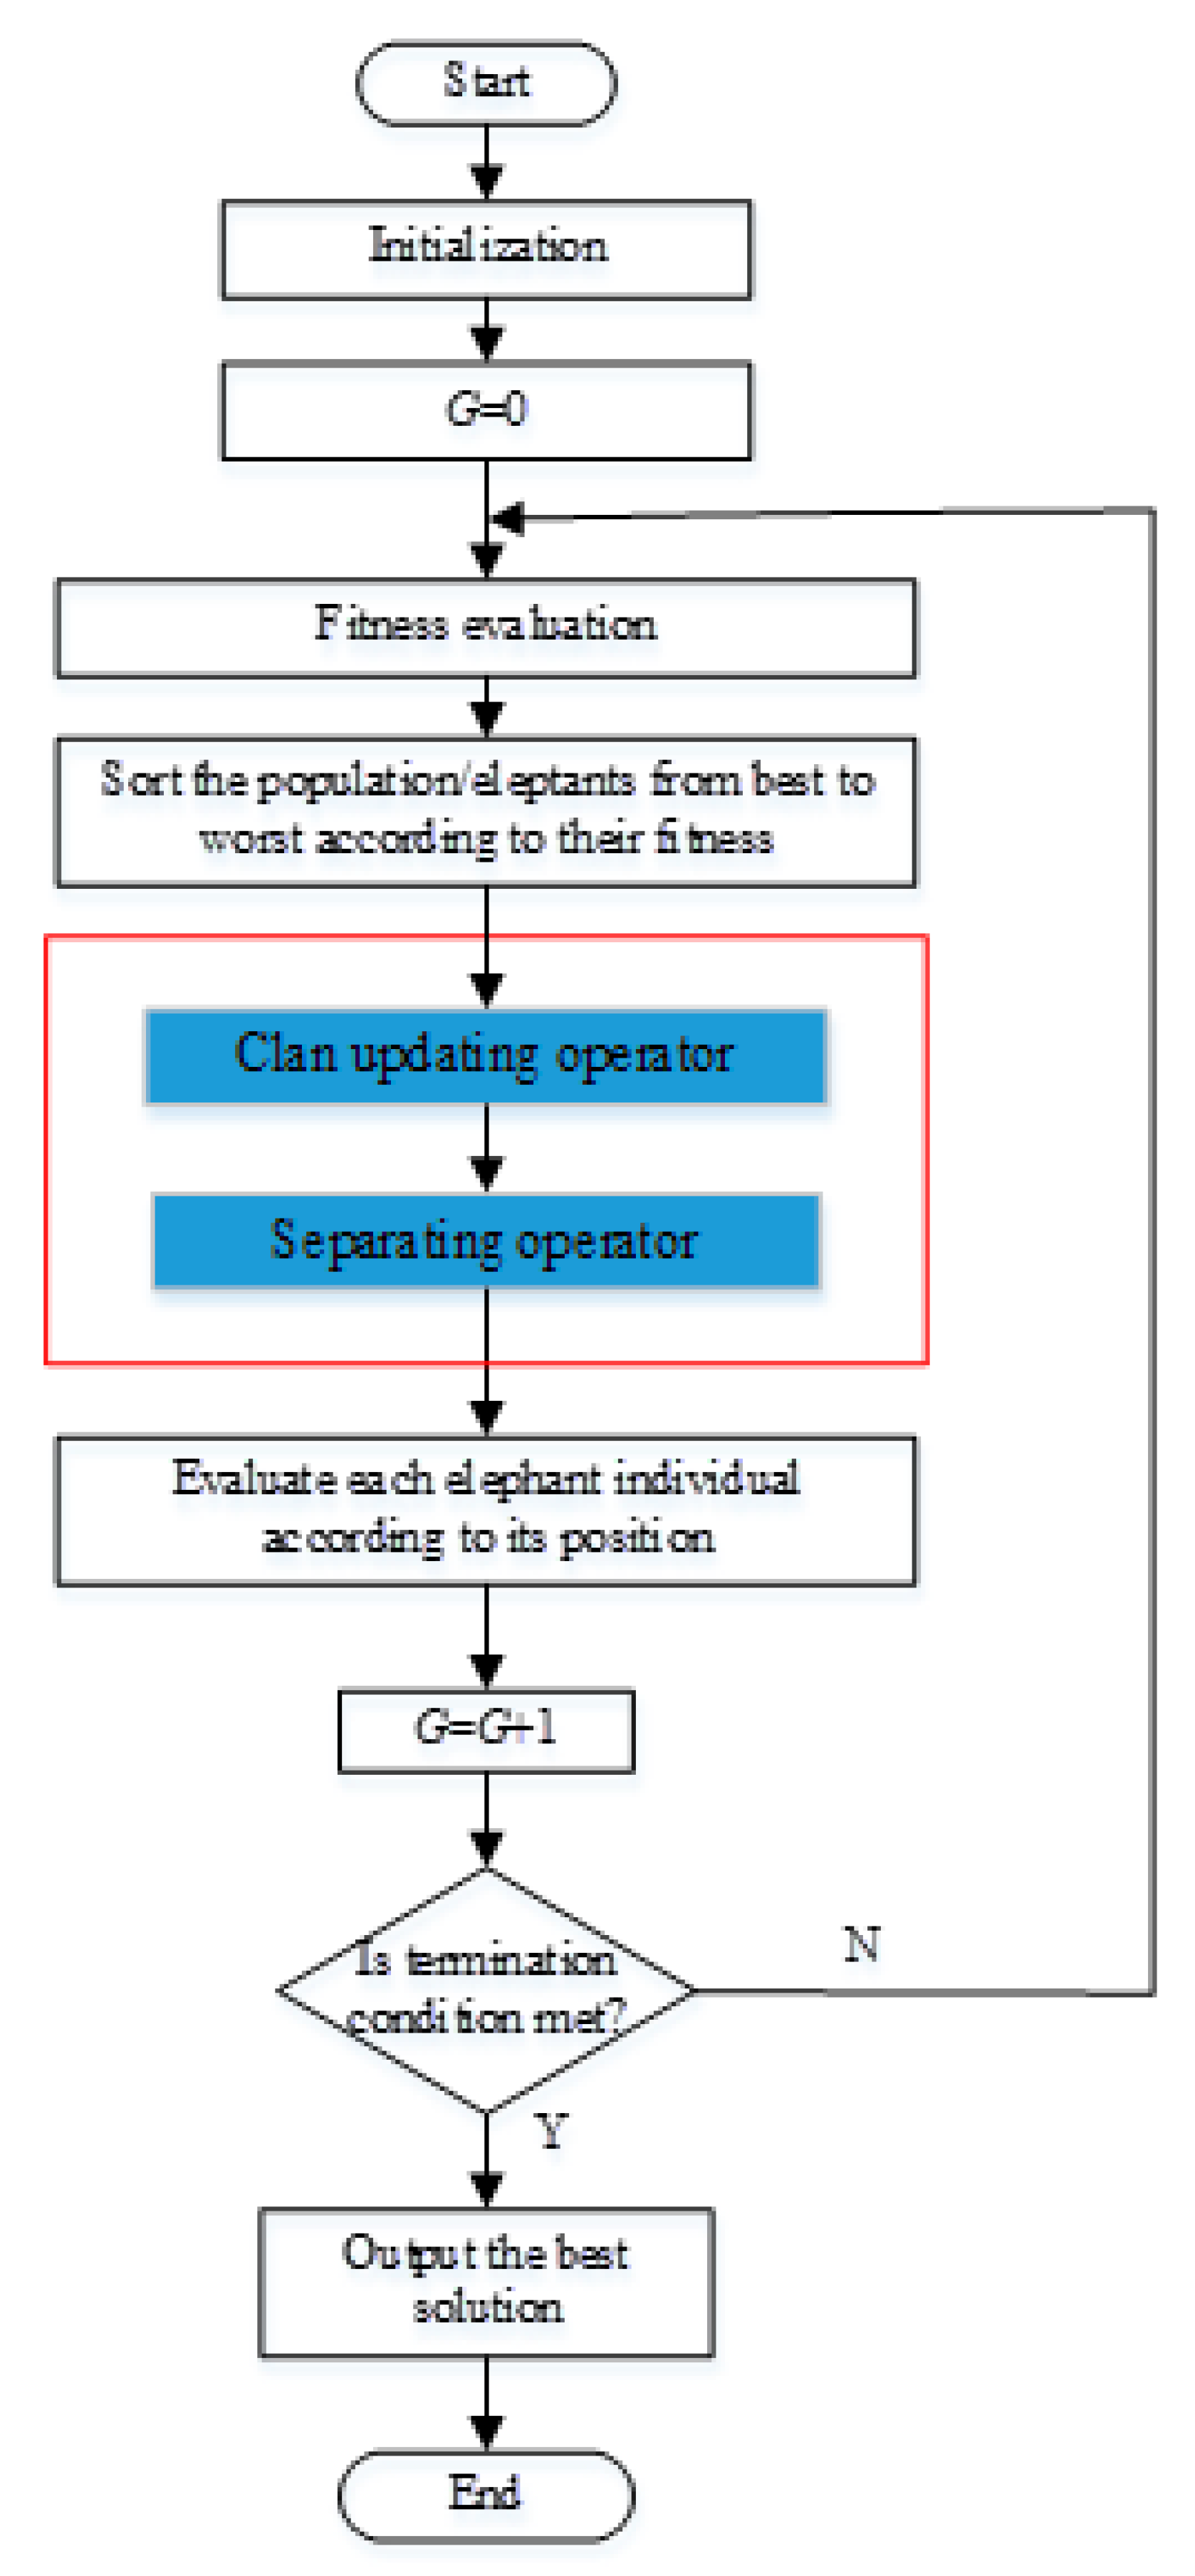
\includegraphics[width=0.3\textwidth]{assets/img/eho_flowchart.png}
        \caption[EHO Flowchart]{\cite[Li et al, S.4]{li_lei_alavi_wang_2020}}
        \label{eho_flowchart}
    \end{center}
\end{figure}
Aus \autoref{eho_clanUpdate} und \autoref{eho_separate} ergibt sich der Ablauf \autoref{eho_flowchart}, der aufzeigt, dass über die Generationen die einzelnen Elefanten immer näher hin zum gesuchten Optimum konvergieren, bis das Endkriterium erreicht ist. Dieses wird durch die maximale Anzahl an Generationen definiert.\\
In \autoref{eho_pseudocode} ist der zugehörige Pseudocode aufgeführt.\\
\begin{figure}[ht]
    \begin{center}
        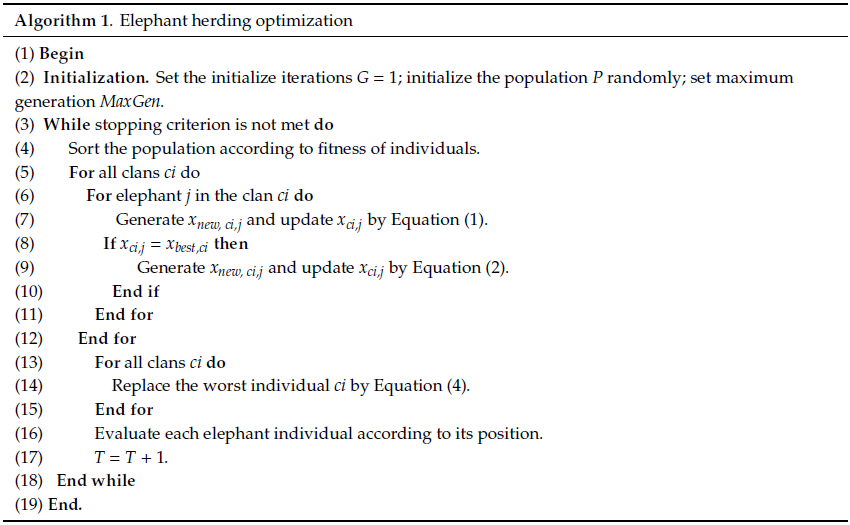
\includegraphics[width=0.7\textwidth]{assets/img/eho_pseudocode.PNG}
        \caption[EHO Pseudocode]{\cite[Li et al, S.5]{li_lei_alavi_wang_2020}}
        \label{eho_pseudocode}
    \end{center}
\end{figure}
Die Elephant Herding Optimization setzt auf eine weitere Unterteilung der Sucher, durch die Aufteilung der Herde in Clans, die als Subgruppen agieren. Dadurch ergibt sich eine höhere Diversität bei der Suche, was zu einer geringeren benötigten Anzahl an Generationen führen kann.\\
Durch die Separierung kann die Konvergenz zum Optimum gezielt erhöht werden, allerdings sollte die Anzahl separierter Tiere nicht höher, als $\frac{n_{ci}}{2}$ liegen, da sonst auch Tiere separiert werden, die zur Zielstrebigkeit des Clans positiv beitragen.  